\documentclass[tikz,border=4pt]{standalone}
\usepackage{amsmath,amssymb}
\usetikzlibrary{arrows.meta}

\begin{document}
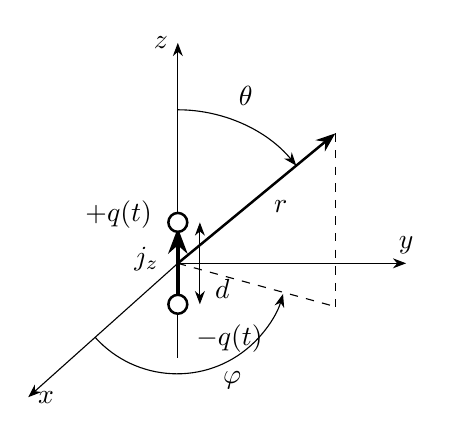
\begin{tikzpicture}[
  >=Stealth,
  font=\normalsize,
  axis/.style={line width=0.4pt},
  curve/.style={line width=0.9pt}
]
  % 3D-like axes
  \draw[axis,->] (0,-1.2) -- (0,2.8) node[left] {$z$};
  \draw[axis,->] (0,0) -- (2.9,0) node[above] {$y$};
  \draw[axis,->] (0,0) -- (-1.9,-1.7) node[right] {$x$};

  % Dipole charges +q(t) and -q(t) on z-axis
  \draw[line width=1.4pt,->] (0,-0.45) -- (0,0.45);
  \fill[white] (0,0.52) circle (0.12);
  \draw[curve] (0,0.52) circle (0.12);
  \fill[white] (0,-0.52) circle (0.12);
  \draw[curve] (0,-0.52) circle (0.12);

  \node[left=3pt] at (-0.1,0.62) {$+q(t)$};
  \node[below right=2pt] at (0.04,-0.58) {$-q(t)$};
  \node[left=2pt] at (-0.05,0.05) {$j_z$};

  % Distance d bracket
  \draw[axis,<->] (0.28,-0.52) -- (0.28,0.52);
  \node[right=2pt] at (0.28,-0.32) {$d$};

  % Observation vector r
  \draw[curve,->] (0,0) -- (2.0,1.65);
  \node[below right] at (1.1,0.92) {$r$};

  % Projection to xy-plane
  \draw[axis,dashed] (2.0,1.65) -- (2.0,-0.55);
  \draw[axis,dashed] (0,0) -- (2.0,-0.55);

  % Angle theta
  \draw[axis,->] (0,1.95) arc (90:39.5:1.95);
  \node[above right] at (0.65,1.88) {$\theta$};

  % Angle phi
  \draw[axis,->] (-1.05,-0.94) arc (-138:-16:1.4);
  \node[below right] at (0.45,-1.25) {$\varphi$};
\end{tikzpicture}
\end{document}
